\documentclass[12pt]{article}

\usepackage{fontspec}
\usepackage{amsmath, amssymb, amsfonts}
\usepackage{graphicx}
\usepackage{hyperref}
\usepackage{color}
\usepackage{geometry}
\geometry{a4paper}

\usepackage{tikz}
\usetikzlibrary{calc, positioning}

\begin{document}
	\begin{minipage}[t]{.5\textwidth}
		{\large Prénom :\\
		Nom :}
	\end{minipage}%
	\begin{minipage}[t]{.5\textwidth}
		\begin{flushright}
			{\Large /30}
		\end{flushright}
	\end{minipage}

	\vspace{3em}
	\begin{center}
			{\Large Examen}\\
			{\large 5e Générale}\\
			18 décembre 2023
	\end{center}
	
	\vspace{3em}
	
	\fbox{\parbox{\linewidth}{%
			\textbf{Consignes :} L'examen commence à 8h10 et se termine à 10h40. Tu as le droit d'avoir une feuille A4 avec les notes que tu auras préparées. Tu peux écrire sur cette feuille ou sur une feuille à part, n'oublie pas de bien écrire tes prénom et nom sur toutes les feuilles que tu utilises. Les machines à calculer sont autorisées. Pose des questions si tu en as besoin. Bon courage !
	}}
	
	\vspace{2em}
	
	\begin{enumerate}
		\item 
			\begin{minipage}[t]{.9\textwidth}
				En avril 1986, de l'iode 131 radioactif a été répandu dans l'air à la suite de l'incendie de l'un des réacteurs de la centrale nucléaire de Tchernobyl.
				Il a été poussé par le vent et s'est répandu sur le sol de toute l'Europe dans des quantités minimes.
				D'un jour à l'autre, la quantité d'iode radioactif diminue de 9,5\%.
				Supposons qu'il soit tombé 100 mg à un endroit donné. Si on désigne par $u_n$ la quantité d'iode radioactif présent le $n^{\text{e}}$ jour, on a donc $u_0 = 1000, u_1 = 905,\dots$
				\begin{enumerate}
					\item Calcule $u_2, \dots, u_5$.
					\item Donne la formule de récurrence qui exprime $u_n$ en fonction de $u_{n-1}$.
					\item Déduis la formule de $u_n$ en fonction de $n$.
				\end{enumerate}
			\end{minipage}%
			\begin{minipage}{.1\textwidth}
				\begin{flushright}
					{\large /3}
				\end{flushright}
			\end{minipage}
			\vspace{1em}
			
		\item 
			\begin{minipage}[t]{.9\textwidth}
				Soit la suite $u$ définie par $u_n = n +3$. Vrai ou faux ? Justifie.
				\begin{enumerate}
					\item La suite $u$ est définie de manière récurrente.
					\item La suite $u$ est croissante.
					\item La suite $u$ est une suite arithmétique.
				\end{enumerate}
			\end{minipage}%
			\begin{minipage}{.1\textwidth}
				\begin{flushright}
					{\large /3}
				\end{flushright}
			\end{minipage}
			\vspace{1em}
			
		\item 
			\begin{minipage}[t]{.9\textwidth}
				Dans ce problème, on va représenter des nombres \textit{triangulaires} en empilant des pions.
				\begin{center}
					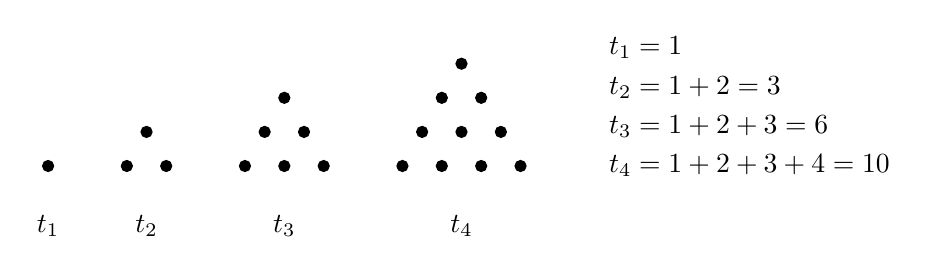
\begin{tikzpicture}
						\filldraw (0,0) circle [radius=2pt];
						\node (initial) at (0,0) {};
						
						\filldraw (initial) ++ (1,0) circle [radius=2pt] node (triangle1bl) {};
						\filldraw (triangle1bl) ++ (0:0.5) circle [radius=2pt] node (triangle1br) {};
						\filldraw (triangle1bl) ++ (60:0.5) circle [radius=2pt];
						
						\filldraw (triangle1br) ++ (1,0) circle [radius=2pt] node (triangle2bl) {};
						\filldraw (triangle2bl) ++ (0:0.5) circle [radius=2pt] node (triangle2bc) {};
						\filldraw (triangle2bl) ++ (0:1) circle [radius=2pt] node (triangle2br) {};
						\filldraw (triangle2bl) ++ (60:0.5) circle [radius=2pt] node (triangle2cl) {};
						\filldraw (triangle2cl) ++ (0:0.5) circle [radius=2pt];
						\filldraw (triangle2cl) ++ (60:0.5) circle [radius=2pt];
						
						\filldraw (triangle2br) ++ (0:1) circle [radius=2pt] node (triangle3bl) {};
						\filldraw (triangle3bl) ++ (0:0.5) circle [radius=2pt];
						\filldraw (triangle3bl) ++ (0:1) circle [radius=2pt];
						\filldraw (triangle3bl) ++ (0:1.5) circle [radius=2pt] node (triangle3br) {};
						\filldraw (triangle3bl) ++ (60:0.5) circle [radius=2pt] node (triangle3mbl) {};
						\filldraw (triangle3bl) ++ (60:1) circle [radius=2pt] node (triangle3mtl) {};
						\filldraw (triangle3bl) ++ (60:1.5) circle [radius=2pt];
						\filldraw (triangle3mbl) ++ (0:0.5) circle [radius=2pt];
						\filldraw (triangle3mbl) ++ (0:1) circle [radius=2pt];
						\filldraw (triangle3mtl) ++ (0:0.5) circle [radius=2pt];
						
						\node at (0,-0.5) [below] {$t_1$};
						\node at (1.25, -0.5) [below] {$t_2$};
						\node at ($(triangle2bc)+(0,-0.5)$) [below] {$t_3$};
						\node at ($(triangle3bl)+(0.75, -0.5)$) [below] {$t_4$};
						
						\node (t4) at ($(triangle3br)+(1,0)$) [right, anchor=west] {$t_4 = 1 + 2 + 3 + 4 = 10$};
						\node at ($(triangle3br)+(1,0.5)$) [right, anchor=west] {$t_3 = 1 + 2 + 3 = 6$};
						\node at ($(triangle3br)+(1,1)$) [right, anchor=west] {$t_2 = 1 + 2 = 3$};
						\node at ($(triangle3br)+(1,1.5)$) [right, anchor=west] {$t_1 = 1$};
					\end{tikzpicture}
				\end{center}
				Le nombre de rangées est noté $n$ ici. On a $t_n$ qui est le nombre total de pions quand on a $n$ rangées, comme représenté sur le schéma ci-dessus.
				\begin{enumerate}
					\item Quel est le nombre de pions de $t_{10}$ ?
					\item Comment peut-on exprimer $t_n$ en fonction de $t_{n-1}$ et de $n$ ?
					\item Comment peut-on exprimer $t_n$ en fonction de $n$ ?
					\item Quel est le nombre triangulaire qui compte 325 pions ?
				\end{enumerate}
			\end{minipage}%
			\begin{minipage}{.1\textwidth}
				\begin{flushright}
					{\large /4}
				\end{flushright}
			\end{minipage}
			\vspace{1em}
			
			\item 
				\begin{minipage}[t]{.9\textwidth}
					Donne la définition d'une suite décroissante.
				\end{minipage}%
				\begin{minipage}{.1\textwidth}
					\begin{flushright}
						{\large /1}
					\end{flushright}
				\end{minipage}
				\vspace{1em}
				
			\item 
				\begin{minipage}[t]{.9\textwidth}
					Soit $u$ une suite décroissante. Quel est le plus grand élément de cette suite~?
				\end{minipage}%
				\begin{minipage}{.1\textwidth}
					\begin{flushright}
						{\large /1}
					\end{flushright}
				\end{minipage}
				\vspace{1em}
				
			\item 
				\begin{minipage}[t]{.9\textwidth}
					Soit la suite $u$ définie par $u_n = 4n-5$. Démontre que cette suite est strictement croissante.
				\end{minipage}%
				\begin{minipage}{.1\textwidth}
					\begin{flushright}
						{\large /5}
					\end{flushright}
				\end{minipage}
				\vspace{1em}
				
			\item 
				\begin{minipage}[t]{.9\textwidth}
					Soit la suite $u$ définie par $u_n = an + 3, ~a \in \mathbb{R}$. Pour quelles valeurs de $a$ la suite $u$ est strictement décroissante ? Explique.
				\end{minipage}%
				\begin{minipage}{.1\textwidth}
					\begin{flushright}
						{\large /3}
					\end{flushright}
				\end{minipage}
				\vspace{1em}
				
			\item 
				\begin{minipage}[t]{.9\textwidth}
					Les suites suivantes sont-elles croissantes ?
					\begin{enumerate}
						\item $u_n = - u_{n-1}; ~u_0 = 3$
						\item $u_n = n^2$
						\item $u_n = -6n + 10$
					\end{enumerate}
				\end{minipage}%
				\begin{minipage}{.1\textwidth}
					\begin{flushright}
						{\large /3}
					\end{flushright}
				\end{minipage}
				\vspace{1em}
				
			\item
				\begin{minipage}[t]{.9\textwidth}
					Soit la suite arithmétique définie par $u_0 = 7$ et $r=2$. Calcule $u_{27}$.
				\end{minipage}%
				\begin{minipage}{.1\textwidth}
					\begin{flushright}
						{\large /1}
					\end{flushright}
				\end{minipage}
				\vspace{1em}
				
			\item
				\begin{minipage}[t]{.9\textwidth}
					Calcule la somme des 212 premiers nombres dont l'écriture se termine par 2 ou 7.
				\end{minipage}%
				\begin{minipage}{.1\textwidth}
					\begin{flushright}
						{\large /3}
					\end{flushright}
				\end{minipage}
				\vspace{1em}
			
			\item
				\begin{minipage}[t]{.9\textwidth}
					Soit $u$ une suite géométrique d'élément initial $u_0$ et de raison $q$.
					\begin{enumerate}
						\item Exprime $u_n$ en fonction de $u_{n-1}$ et de $u_{n+1}$.
						\item Les nombres 20, $z$, 180 sont trois termes consécutifs d'une suite géométrique. Calcule $z$.
					\end{enumerate}
				\end{minipage}%
				\begin{minipage}{.1\textwidth}
					\begin{flushright}
						{\large /3}
					\end{flushright}
				\end{minipage}
				\vspace{1em}
			
	\end{enumerate}
	
\end{document}